\documentclass[tikz, border=10pt]{standalone}

\usepackage{amssymb}
\usetikzlibrary{positioning, fit, backgrounds, arrows.meta, calc, shapes.geometric}

\begin{document}

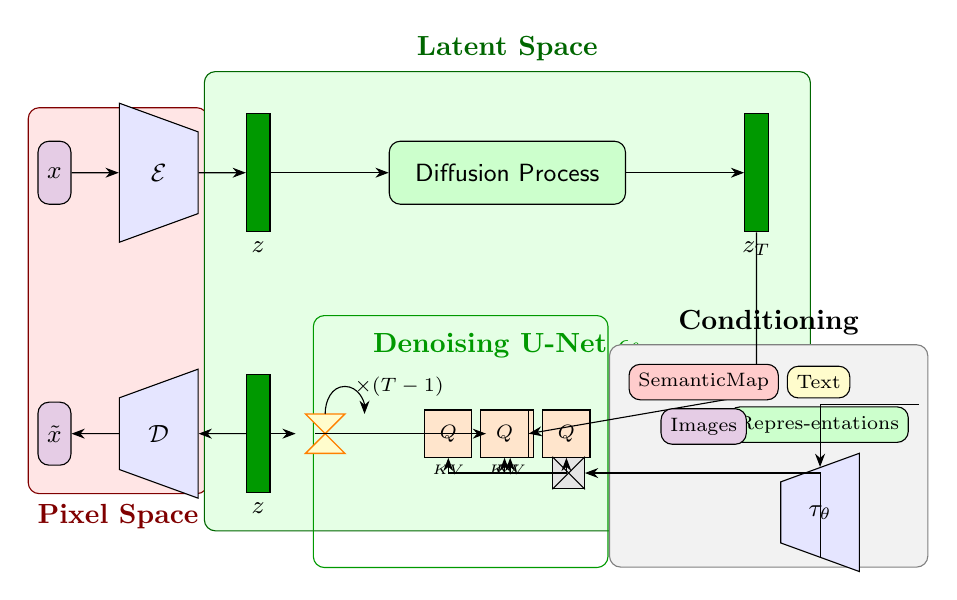
\begin{tikzpicture}[%
    font=\sffamily\small,
    >=Stealth,
    node distance=1cm,
    % Colors
    latentfill/.style={fill=green!10, draw=green!40!black},
    pixelfill/.style={fill=red!10, draw=red!50!black},
    condfill/.style={fill=gray!10, draw=gray},
    block/.style={draw, rectangle, rounded corners, fill=white, minimum height=0.8cm, align=center},
    tensor/.style={draw, fill=green!60!black, minimum width=0.3cm, minimum height=1.5cm},
    kvbox/.style={draw, fill=orange!20, rectangle, minimum size=0.6cm, font=\scriptsize},
    switch/.style={draw, fill=black!20, circle, inner sep=2pt},
    % Macros for complex shapes
    trapezium_enc/.style={draw, trapezium, trapezium angle=70, shape border rotate=270, fill=blue!10, minimum height=1cm},
    trapezium_dec/.style={draw, trapezium, trapezium angle=70, shape border rotate=90, fill=blue!10, minimum height=1cm}
]

% --- 1. Pixel Space (Left) ---
\node[block, fill=violet!20] (x) {$x$};
\node[trapezium_enc, right=0.6cm of x] (E) {$\mathcal{E}$};
\node[tensor, right=0.6cm of E, label=below:$z$] (z) {};
\node[block, fill=violet!20, below=2.5cm of x] (xtilde) {$\tilde{x}$};
\node[trapezium_dec, right=0.6cm of xtilde] (D) {$\mathcal{D}$};
\node[tensor, right=0.6cm of D, label=below:$z$] (z_hat) {};

% Connections
\draw[->] (x) -- (E);
\draw[->] (E) -- (z);
\draw[->] (D) -- (xtilde);
\draw[->] (z_hat) -- (D);

% --- 2. Latent Space Main Process ---
\node[block, fill=green!20, right=1.5cm of z, minimum width=3cm] (diff) {Diffusion Process};
\node[tensor, right=1.5cm of diff, label=below:$z_T$] (zT) {};

\draw[->] (z) -- (diff);
\draw[->] (diff) -- (zT);

% --- 3. Denoising U-Net (Center Bottom) ---
% Define U-Net Area Coordinates
\coordinate (unet_c) at ($(z_hat)!0.5!(zT |- z_hat)$); % Center
\coordinate (unet_l) at ($(z_hat)+(1.2,0)$);
\coordinate (unet_r) at ($(zT |- z_hat)+(-1.2,0)$);

% Draw U-Net Background manually for stability
\begin{scope}[on background layer]
    \draw[fill=blue!10, draw=blue!50!black] 
        ($(unet_l)+(0,1.2)$) -- ($(unet_l)+(1.5,0.5)$) -- 
        ($(unet_r)+(-1.5,0.5)$) -- ($(unet_r)+(0,1.2)$) -- 
        ($(unet_r)+(0,-1.2)$) -- ($(unet_r)+(-1.5,-0.5)$) -- 
        ($(unet_l)+(1.5,-0.5)$) -- ($(unet_l)+(0,-1.2)$) -- cycle;
    % Dashed connections
    \draw[dashed, gray] ($(unet_l)+(1.5,0)$) -- ($(unet_r)+(-1.5,0)$);
\end{scope}

% QKV Blocks
\node[kvbox] (qkv1) at ($(unet_l)+(2.0,0)$) {$Q$};
\node[kvbox, right=0.1cm of qkv1] (qkv2) {$Q$};
\node[kvbox] (qkv4) at ($(unet_r)+(-2.0,0)$) {$Q$};
\node[kvbox, left=0.1cm of qkv4] (qkv3) {$Q$};

% Label KV inside
\node[font=\tiny, below=-1pt] at (qkv1.south) {$KV$};
\node[font=\tiny, below=-1pt] at (qkv2.south) {$KV$};
\node[font=\tiny, below=-1pt] at (qkv3.south) {$KV$};
\node[font=\tiny, below=-1pt] at (qkv4.south) {$KV$};

% Denoising Step Icon (Bowtie)
\node (bowtie) at ($(unet_l)!0.5!(z_hat)$) {};
\draw[fill=yellow!20, draw=orange, line width=0.5pt] 
    ($(bowtie)+(0,0.25)$) -- ($(bowtie)+(0.5,-0.25)$) -- 
    ($(bowtie)+(0,-0.25)$) -- ($(bowtie)+(0.5,0.25)$) -- cycle;

% Switch Icon
\node[draw, fill=black!10, rectangle, minimum size=0.4cm, right=0.3cm of qkv4, yshift=-0.5cm] (switch) {};
\draw (switch.south west) -- (switch.north east);
\draw (switch.north west) -- (switch.south east);

% Connections U-Net
\draw[->] (zT) -- ($(zT |- unet_r)+(0,0.5)$) -- (qkv4.east);
\draw[->] (z_hat) -- (bowtie);
\draw[->] (bowtie) -- (qkv1);

% Loop z_T-1
\draw[->] ($(bowtie)+(0.25,0.25)$) to[out=90,in=180] ($(bowtie)+(0.5,0.6)$) node[right, font=\scriptsize] {$\times(T-1)$} to[out=0,in=90] ($(bowtie)+(0.75,0.25)$);

% --- 4. Conditioning (Right) ---
\node[trapezium_dec, right=1.5cm of unet_r, yshift=-1cm] (tau) {$\tau_\theta$};

% Conditioning inputs
\node[draw, fill=red!20, rounded corners, font=\scriptsize, above left=1cm and 0.1cm of tau] (c_sem) {Semantic\\Map};
\node[draw, fill=yellow!20, rounded corners, font=\scriptsize, right=0.1cm of c_sem] (c_txt) {Text};
\node[draw, fill=green!20, rounded corners, font=\scriptsize, below=0.1cm of c_txt] (c_rep) {Repres-\\entations};
\node[draw, fill=violet!20, rounded corners, font=\scriptsize, below=0.1cm of c_sem] (c_img) {Images};
\node[fit=(c_sem)(c_txt)(c_rep)(c_img)](c_group){};

% Connections
\draw[->] (c_group) -| (tau.north);
\draw[->] (tau.south) |- (switch.east);

\draw[->] (switch) -| (qkv4.south);
\draw[->] (switch) -| (qkv3.south);
\draw[->] (switch) -| (qkv2.south);
\draw[->] (switch) -| (qkv1.south);

% --- Background Regions ---
\begin{scope}[on background layer]
    % Pixel Space
    \node[fit=(x)(xtilde)(E)(D), pixelfill, rounded corners, label={[text=red!50!black, font=\bfseries]south:Pixel Space}] {};

    % Latent Space
    \node[fit=(z)(zT)(diff)(unet_l)(unet_r)(switch), latentfill, rounded corners, inner sep=15pt, label={[text=green!40!black, font=\bfseries]north:Latent Space}] (bg_latent) {};

    % Inner Green Box for U-Net
    \draw[green!60!black, rounded corners] ($(unet_l)+(-0.5,1.5)$) rectangle ($(switch)+(0.5,-1.2)$);
    \node[text=green!60!black, font=\bfseries, anchor=north] at ($(unet_c)+(0,1.4)$) {Denoising U-Net $\epsilon_\theta$};

    % Conditioning
    \node[fit=(c_group)(tau), condfill, rounded corners, label={[text=black, font=\bfseries]north:Conditioning}] {};
\end{scope}

\end{tikzpicture}

\end{document}
